\documentclass[main.tex]{subfiles}
\usepackage[utf8]{inputenc}
\usepackage[
backend=biber,
style=alphabetic,
sorting=ynt
]{biblatex}
\usepackage{subfiles}

\addbibresource{../references.bib} %Imports bibliography file

% Document information
\title{Proceso}
\author{Rocío Mena}
\date{\today}

\begin{document}

\maketitle

\section{Objetivos del Plan de Tesina Final de Carrera}

El objetivo general de este plan de tesina final de carrera es el \textbf{uso de blockchain} como tecnología de vanguardia para el desarrollo de una \textbf{aplicación prototipo} destinada a \textbf{mejorar la trazabilidad} en modelos de economía circular orientados al \textbf{reciclado de vidrio}.

Como objetivos específicos que aportan al trabajo final de tesina se puede mencionar:

\begin{itemize}
    \item Entender los procesos de adopción de tecnologías tales como blockchain y las capacidades actuales en la región para el uso de sistemas de trazabilidad.
    \item En todo lo referido a las Ciencias de la Computación, se busca que la alumna pueda desarrollar una aplicación prototipo funcional basada en tecnología blockchain. Esto permitirá la trazabilidad transparente, segura y en tiempo real de la gestión de residuos, en particular el vidrio, desde su generación hasta su disposición final, con el fin de garantizar el cumplimiento normativo, mejorar la eficiencia operativa y aumentar la confianza entre todos los actores involucrados en el proceso.
\end{itemize}

El desarrollo de esta aplicación prototipo se fundamenta en la necesidad de abordar los desafíos de la trazabilidad en los procesos de reciclaje de vidrio, dentro del marco de la economía circular. La elección de un prototipo se justifica por la viabilidad de mostrar una solución tangible al problema planteado, dentro del alcance esperado de un trabajo final de tesina. Un prototipo funcional permite demostrar las capacidades y ventajas de la tecnología propuesta, así como validar la solución en un entorno controlado antes de avanzar a una implementación más amplia.

La elección de blockchain como tecnología de base se debe a sus características inherentes de inmutabilidad, transparencia y descentralización, que permiten garantizar la integridad de los datos en tiempo real. Estas cualidades facilitan la colaboración entre los diferentes actores de la cadena de suministros, al proporcionar un acceso confiable y seguro a la información sobre la gestión de los residuos. Además, la descentralización de la información permite eliminar intermediarios, mejorar la eficiencia y reducir riesgos de manipulación de datos.

El reciclado de vidrio se seleccionó como caso de estudio debido a su amplio uso en la industria de alimentos y bebidas, su capacidad de reciclaje al 100\%, y los desafíos específicos que enfrenta en la región de Mendoza, donde el proceso es complejo e ineficiente, involucrando a múltiples actores y etapas. Al aplicar soluciones tecnológicas basadas en blockchain, buscamos optimizar la trazabilidad y eficiencia del proceso, generando un impacto positivo tanto en el medio ambiente como en la economía local.

La trazabilidad se ha identificado como un aspecto clave en la gestión de residuos, ya que permite conocer el origen, destino, composición y estado de los residuos en cada etapa del proceso. Contar con esta información facilita la toma de decisiones, permite la identificación temprana de problemas y promueve la mejora continua por parte de los actores involucrados.

La elección de la economía circular como enfoque para el desarrollo del prototipo refuerza el compromiso con la sostenibilidad, promoviendo la reutilización y reciclado de materiales, lo que minimiza el desperdicio y maximiza el valor a lo largo del ciclo de vida de los productos. Este modelo contribuye a la sostenibilidad no solo ambiental, sino también económica y social.

El cumplimiento normativo es otro aspecto crítico para la adopción de nuevos sistemas de reciclaje, debido a que las leyes y regulaciones ambientales establecen requisitos legales para la protección del medio ambiente y la salud pública. Contar con un sistema de trazabilidad basado en blockchain permite verificar el cumplimiento de las normativas vigentes, facilitando la comercialización de productos reciclados y garantizando la transparencia de la información.

En términos de eficiencia operativa, la mejora de la trazabilidad incide directamente en la reducción de costos, tiempos y errores en la gestión de residuos. Esto se traduce en una mayor productividad, competitividad y rentabilidad para los actores de la cadena de suministro, promoviendo una gestión más efectiva y ágil.

Por último, la confianza entre los actores de la cadena de suministros es un factor determinante para el éxito de cualquier iniciativa de reciclaje. La opacidad de la información en los sistemas actuales genera desconfianza, conflictos y pérdidas. Al utilizar blockchain, se proporciona una visión clara y confiable de la información relevante, fomentando la colaboración, coordinación y comunicación entre los actores, mejorando así la gestión integral del reciclaje.

/subsection{Alcance del Proyecto}

El presente trabajo de tesina se centra en la \textbf{investigación y desarrollo de un prototipo de aplicación} basado en tecnología blockchain, cuyo propósito es mejorar la trazabilidad en los modelos de economía circular aplicados al reciclado de vidrio. 

El sistema diseñado permitirá registrar y auditar las transacciones de los residuos de vidrio a lo largo de toda la cadena de suministro, abarcando desde su generación hasta su disposición final. El enfoque principal de este prototipo será la trazabilidad en la \textbf{cadena de producción de envases de vidrio}, posponiendo para futuras implementaciones la integración con otros actores involucrados en el reciclado de vidrio.

\begin{figure}[h]
    \centering
    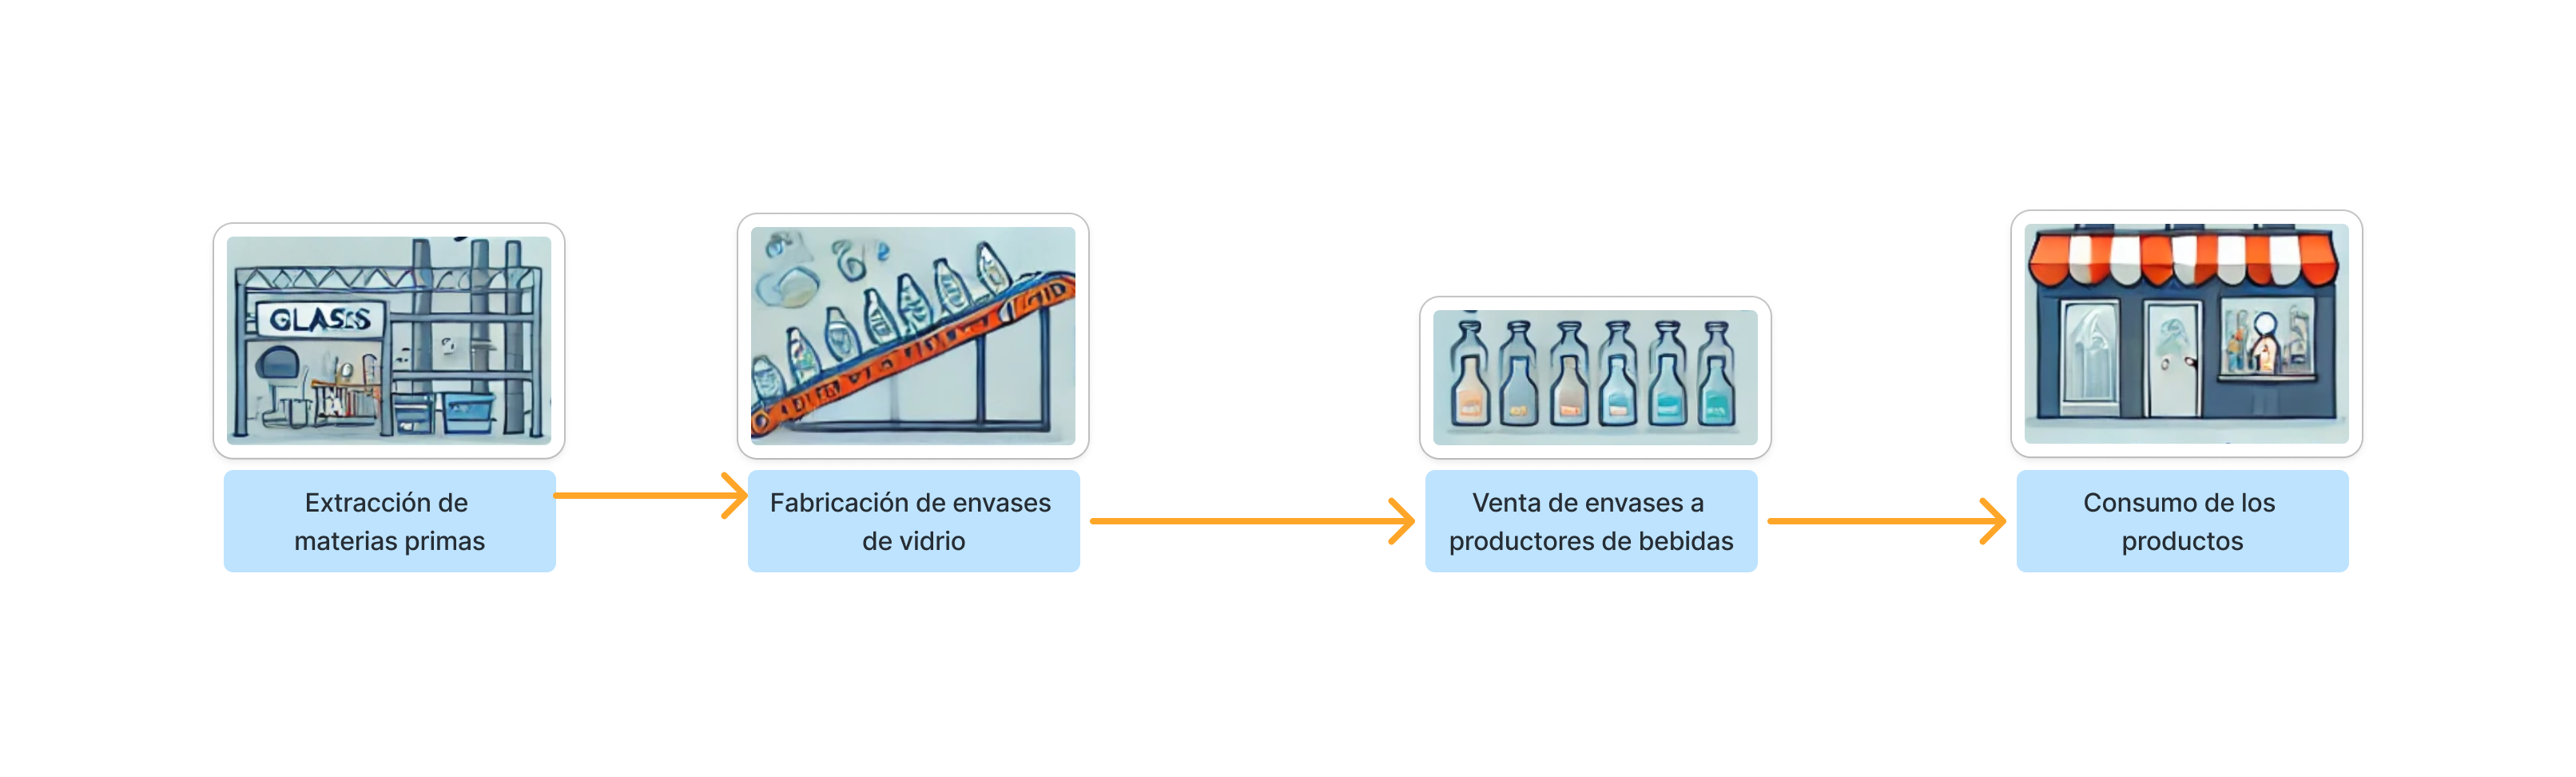
\includegraphics[width=0.8\textwidth]{../assets/glass-production.png}
    \caption{Diagrama del proceso de producción de envases de vidrio.}
    \label{fig:glass_production}
\end{figure}

El enfoque en la cadena de producción de envases de vidrio se justifica en función de los resultados obtenidos en la investigación del estado del arte. Se identificó que en esta primera fase de la cadena no existen soluciones tecnológicas locales que aborden de manera efectiva el problema de la trazabilidad. Por otro lado, en las fases posteriores, como la recolección y el reciclado, ya se han implementado soluciones tecnológicas que mejoran la adopción y eficiencia de los procesos, y que podrán ser integradas en futuras fases del proyecto.

\subfile{methodology}

\end{document}
